\documentclass{article}
\usepackage[final]{neurips_2023}
\usepackage[numbers]{natbib}
\usepackage{amsmath, amssymb}
\usepackage{subcaption}
\usepackage{graphicx}
\usepackage{booktabs}
\usepackage{algorithm}
\usepackage{algorithmic}
\usepackage{tikz}
\usepackage{pgfplots}
\pgfplotsset{compat=1.18}

\title{Hierarchical Transfer Learning for Fine-Grained Animal Classification}

\author{%
  Robert Berman \quad Ahmed Taeha \quad Darren Chan\\
  Columbia University\\
  \texttt{\{rb3578, at4058, dc3816\}@columbia.edu}%
}

\begin{document}

\maketitle

\begin{abstract}
We study hierarchical image classification (super-class: bird/dog/reptile; sub-class: 88 fine-grained labels) under distribution shift and novel sub-classes. We benchmark vision-only and vision-language transfer learning models, compare freezing vs.\ finetuning, and evaluate augmentation/regularization. A frozen CLIP model delivers the best novel super-class accuracy at 89.72\% while a simple ResNet-50 finetune delivers the best novel sub-class accuracy of 64.17\%. We release configs, checkpoints, and scripts for reproducibility.
\end{abstract}

\section{Introduction}
Hierarchical classification requires predicting both coarse (super-class) and fine-grained (sub-class) labels. Distribution shifts and unseen sub-classes complicate transfer from generic pretraining. We evaluate whether vision-language encoders (CLIP, SigLIP) outperform a strong vision baseline (ResNet-50) and whether freezing, finetuning, and augmentation meaningfully affect robustness.

\section{Related Work}
\textbf{Transfer learning for vision.} CNN backbones such as ResNet-50 have long served as strong finetuning baselines \citep{he2016resnet}. ResNets address core issues with deep convolutional architectures that make optimization difficult, where deeper networks experience accuracy saturation and subsequent degradation. Through the use of residual connections, the inputs to the network are directly propagated to deeper layers using identity mappings which mitigate issues of vanishing gradients and optimization instabilities. ResNet models are pretrained on ImageNet-1k, consisting of 1.28 million images with 1,000 classes which acts as a flexible and generalized baseline for downstream tasks in image classification. In transfer learning, early layers are typically frozen to keep the model remembering the low level features it was trained on, while the deeper layers will be updated and tailored to the new task or domain along with a new classification head.

\textbf{Vision-language pretraining.} Models such as CLIP \citep{radford2021clip} and SigLIP \citep{zhai2023siglip} learn joint image-text embeddings, capturing both visual and semantic relationships in a shared latent space. Through a contrastive learning objective, CLIP trains both an image encoder and a text encoder and attempts to bring the matching image-text embeddings closer while pushing them further from incorrect pairings. Instead of a softmax-based contrastive loss, SigLIP uses pairwise sigmoidal loss to reduce memory and computation. Both CLIP and SigLIP have the strong ability for zero-shot image classification due to the relationships between the image and text, which allows them to match images to textual descriptions directly. The impact of unseen classes is then mitigated since CLIP and SigLIP match through text embeddings even if images were not explicitly seen during training.

\textbf{Regularization and augmentation.} Mixup \citep{zhang2018mixupempiricalriskminimization} augments the training data through linear interpolations between the input data and their corresponding labels, encouraging smoother decision boundaries. Dropout \citep{JMLR:v15:srivastava14a} randomly deactivates network units during training, encouraging the model to learn more complex representations throughout the network. Weight decay applies an L2 regularization to the model, controlling model complexity and penalizing large weights. These regularization methods improve robustness and stability during training, leading to better performance under distribution shifts and on unseen data. RandAugment \citep{cubuk2019randaugment} is a data augmentation method that aids in increasing diversity within the training data by adding variations through random transformations and distortions. With augmentations such as rotations, color adjustments, and translations, models are encouraged to learn the invariances to common perturbations that arise in each class. All these methods are complementary regularization techniques which can be used to mitigate overfitting and improve generalization. 

\section{Method}
\subsection{Model heads and loss}
All models share an encoder producing a feature vector fed to two linear heads: one for super-class and one for sub-class. For logits $z^{(s)}, z^{(f)}$ and targets $y^{(s)}, y^{(f)}$ we optimize
\begin{equation}
\mathcal{L} = \tfrac{1}{2}\,\text{CE}(z^{(s)}, y^{(s)}) + \tfrac{1}{2}\,\text{CE}(z^{(f)}, y^{(f)}),
\end{equation}
optionally with mixup on inputs/labels.

\subsection{Training setup}
AdamW optimizer, cosine LR with warmup, batch size 32, image size 224, grad clip 1.0. Augmentation: random resized crop, RandAugment; mixup and dropout per configuration. Devices: Apple M3 Max (MPS).

\subsection{Thresholding for novel classes}
To identify potential novel super-classes and sub-classes for the test set, we leveraged a model confidence threshold. Using the validation set, we computed confidence scores using the maximum softmax probabilities for each sample at both the super-class and sub-class levels. At inference, an image was flagged as a novel class if its predicted confidence fell below the corresponding model and threshold.

\subsection{Algorithms}
\begin{algorithm}[h]
\caption{Freeze vs.\ Finetune Sweep (per config)}
\begin{algorithmic}[1]
\STATE Load config, set seed, build loaders
\STATE Build encoder + dual heads (freeze or train encoder)
\FOR{epoch $1..E$}
    \STATE Train with mixed precision; apply mixup if enabled
    \STATE Validate; track best metrics
    \STATE Save checkpoint
\ENDFOR
\end{algorithmic}

\end{algorithm}
\begin{algorithm}[H]
\caption{Novelty Threshold Computation (Super \& Sub Classes)}
\begin{algorithmic}[1]
\STATE Initialize empty confidence lists
\FOR{each batch in validation loader}
    \STATE Compute logits $(\mathbf{L}_{super}, \mathbf{L}_{sub})$
    \STATE Apply softmax to obtain probabilities
    \STATE Extract maximum probability per sample as confidence
    \STATE Append super-class and sub-class confidences
\ENDFOR
\STATE confsuper, confsub $=$ threshold as n-th percentile of super-class and sub-class confidence lists
\STATE \textbf{return} (conf\_super, conf\_sub)
\end{algorithmic}
\end{algorithm}


\section{Data and Metrics}
The dataset provided (COMS 4776 transfer-learning set) included (6{,}288 labeled samples), 3 super-classes + potential novel; 88 sub-classes. Validation split counts: bird 185, dog 194, reptile 227. Metrics: super/sub accuracy, joint accuracy (both correct), macro F1 for super and sub.

\section{Experiments}
We evaluate:
\begin{itemize}
    \item \textbf{Baselines:} ResNet-50 finetune; CLIP ViT-B/32 frozen; SigLIP ViT-B/16 frozen.
    \item \textbf{Finetune sweeps:} CLIP ViT-B/32, SigLIP ViT-B/16; ResNet frozen.
    \item \textbf{Aug/regularization:} mixup, dropout, weight decay variations for ResNet/CLIP/SigLIP.
\end{itemize}

\subsection{Results}
\begin{table}[h]
\centering
\begin{tabular}{lcccc}
\toprule
Run & Super Acc & Sub Acc & Joint Acc & Sub F1 \\
\midrule
ResNet-50 (finetune) & 1.0000 & \textbf{0.9785} & \textbf{0.9785} & \textbf{0.9673} \\
ResNet-50 (aug/mixup) & 1.0000 & 0.9785 & 0.9785 & 0.9626 \\
CLIP ViT-B/32 (finetune) & 1.0000 & 0.9719 & 0.9719 & 0.9566 \\
SigLIP ViT-B/16 (finetune) & 1.0000 & 0.9769 & 0.9769 & 0.9591 \\
CLIP ViT-B/32 (frozen) & 1.0000 & 0.9554 & 0.9554 & 0.9372 \\
CLIP ViT-B/32 (aug) & 1.0000 & 0.9472 & 0.9472 & 0.9249 \\
ResNet-50 (frozen) & 0.9901 & 0.8482 & 0.8416 & 0.8173 \\
SigLIP ViT-B/16 (frozen) & 0.9917 & 0.6865 & 0.6815 & 0.5776 \\
SigLIP ViT-B/16 (aug) & 0.9868 & 0.6502 & 0.6403 & 0.5360 \\
\bottomrule
\end{tabular}
\caption{Validation metrics across runs. Best sub-class performance from ResNet-50 finetune; SigLIP finetune close. Augmentation helped modestly or matched baselines; frozen encoders underperform.}
\end{table}

\begin{table}[H]
\centering

\begin{tabular}{lccc}
\toprule
Run & Super Acc & Seen Super Acc & Unseen Super Acc \\
\midrule
CLIP ViT-B/32 (frozen) & 0.9348 & 0.9496 & 0.8972 \\ 
CLIP ViT-B/32 (finetune) & 0.9174 & 0.9687 & 0.7870 \\
SigLIP ViT-B/16 (finetune) & 0.9082 & 0.9719 & 0.7465 \\
ResNet-50 (finetune) & 0.8932 & 0.9281 & 0.8047 \\
ResNet-50 (aug/mixup) & 0.8757 & 0.9569 & 0.6696 \\
\bottomrule
\end{tabular}

\vspace{0.6em}

\begin{tabular}{lccc}
\toprule
Run & Sub Acc & Seen Sub Acc & Unseen Sub Acc \\
\midrule
ResNet-50 (aug/mixup) & 0.7013 & 0.9218 & 0.6417 \\
CLIP ViT-B/32 (frozen) & 0.6535 & 0.9108 & 0.5840 \\ 
SigLIP ViT-B/16 (finetune) & 0.6114 & 0.9340 & 0.5244 \\
CLIP ViT-B/32 (finetune) & 0.6105 & 0.9260 & 0.5253 \\
ResNet-50 (finetune) & 0.5821 & 0.9419 & 0.4849 \\
\bottomrule
\end{tabular}

\caption{Test accuracies on super-classes and sub-classes based on the best best models}
\end{table}

\subsection{Training curves and confusion}
Figure~\ref{fig:curves} shows ResNet-50 validation loss and sub-class accuracy over epochs (representative run). Loss drops rapidly and sub-class accuracy stabilizes above 0.95. Table~\ref{tab:confusion} reports super-class confusion for the best model; no super-class errors were observed.

\begin{figure}[h]
\centering
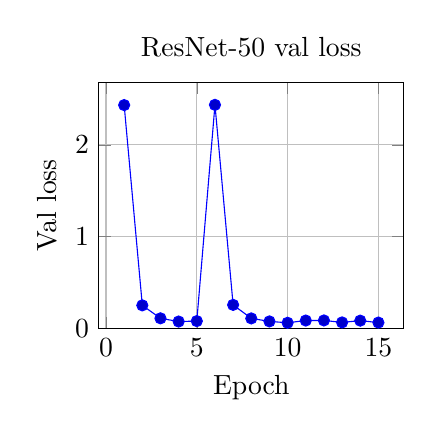
\begin{tikzpicture}
\begin{axis}[
    width=0.45\linewidth,
    xlabel=Epoch,
    ylabel=Val loss,
    title={ResNet-50 val loss},
    ymin=0, grid=both]
\addplot coordinates {
(1,2.4331)(2,0.2523)(3,0.1112)(4,0.0762)(5,0.0810)
(6,2.4355)(7,0.2575)(8,0.1102)(9,0.0776)(10,0.0627)
(11,0.0870)(12,0.0881)(13,0.0666)(14,0.0859)(15,0.0649)
};
\end{axis}
\end{tikzpicture}
\hfill
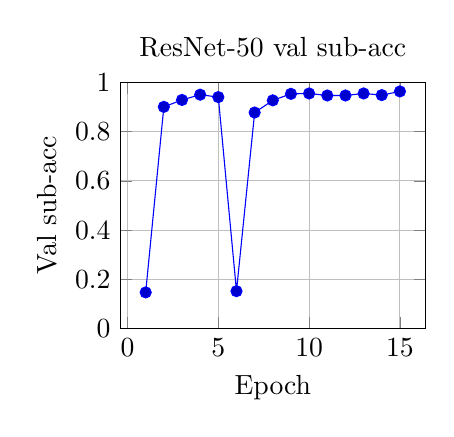
\begin{tikzpicture}
\begin{axis}[
    width=0.45\linewidth,
    xlabel=Epoch,
    ylabel=Val sub-acc,
    title={ResNet-50 val sub-acc},
    ymin=0, ymax=1, grid=both]
\addplot coordinates {
(1,0.1469)(2,0.9010)(3,0.9290)(4,0.9505)(5,0.9406)
(6,0.1518)(7,0.8779)(8,0.9274)(9,0.9538)(10,0.9554)
(11,0.9472)(12,0.9472)(13,0.9554)(14,0.9488)(15,0.9637)
};
\end{axis}
\end{tikzpicture}
\caption{Validation curves for ResNet-50 finetune.}
\label{fig:curves}
\end{figure}

\begin{table}[h]
\centering
\begin{tabular}{lccc}
\toprule
 & Pred bird & Pred dog & Pred reptile \\
\midrule
True bird & 185 & 0 & 0 \\
True dog & 0 & 194 & 0 \\
True reptile & 0 & 0 & 227 \\
\bottomrule
\end{tabular}
\caption{Super-class confusion (ResNet-50 finetune).}
\label{tab:confusion}
\end{table}

\subsection{Error analysis}
CLIP finetune misclassified 27 validation samples (see \texttt{outputs/clip\_vitb32\_errors.csv}); most errors are fine-grained sub-class confusions within the correct super-class.

\subsection{Robustness}
Overall robustness on CLIP finetune: super\_acc 1.0, sub\_acc 0.9554, joint\_acc 0.9554. Novel sub-class labels were not provided in the dataset; the robustness script supports filtering when available; robustness to true novel sub-classes remains a limitation.

\section{Discussion}
Our experiments on the given models highlight several key findings regarding hierarchical transfer learning for fine-grained animal classification:

\textbf{ResNet-50 as a strong baseline:} Despite the availability of more advanced vision-language models like CLIP and SigLIP, a simple ResNet-50 finetune achieved the best sub-class accuracy (97.85\%) and joint accuracy (97.85\%) in our validation metrics. For test metrics when identifying novel super-classes, a finetuned ResNet performed in the middle between CLIP and SigLIP with an accuracy of 80.47\%. The seen super-classes performed slightly below at 92.81\%. While finetuned ResNet performed the best for novel sub-class accuracies at 64.17\%, it struggled with 48.49\% unseen accuracy depending on the training methods. This result shows the effectiveness of vision-only models when fine-tuned on domain-specific data, especially when the dataset size is moderate and the task is well-aligned with the pre-training distribution.

\textbf{Finetuning vs.\ freezing:} Across all models, finetuning the encoder consistently outperformed freezing it when novel classes were not considered. This suggests that adapting the entire model to the target dataset is critical for achieving high accuracy, especially for fine-grained sub-class distinctions. Frozen encoders, while computationally efficient, struggled to match the performance of their fine-tuned counterparts, particularly for sub-class accuracy. When considering novel classes and the models we chose, the frozen CLIP model outperformed all finetuned variations with a unseen super-class accuracy of 89.72\% and unseen sub-class accuracy of 58.40\%. This indicates that by not freezing, the models adapted more towards the domain of all the seen classes and performed better, but there was an apparent trade-off to generalization when requiring a prediction of novelty.

\textbf{Impact of augmentation and regularization:} Techniques like mixup, dropout, and RandAugment provided modest or neutral gains in most cases. For ResNet-50, augmentation did not significantly improve performance beyond the baseline finetune. This indicates that the model's robustness to distribution shifts and fine-grained distinctions were already strong, and additional augmentation had limited impact. However, when predicting novel classes, augmentation and regularization and a larger impact with ResNet-50, having it perform the best for novel sub-class detection with a 64.17\% novel sub-class accuracy. For the novel super-classes, it struggled with a 66.96\% accuracy, which could indicate it was better at identifying known super-class/novel sub-class variations. These methods of augmentation and regularization demonstrate that they still enhance the ability to generalize, which allows the models to identify these variations that may fall outside the distribution which aided in the strong sub-class predictions.

\textbf{Vision-language models:} CLIP and SigLIP demonstrated strong performance, but they did not always surpass ResNet-50 in this specific task. Within validation metrics, CLIP finetune achieved a sub-class accuracy of 97.19\%, slightly below ResNet-50, while SigLIP finetune reached 97.69\%. Frozen CLIP performed the best in unseen super-class detection with a 89.72\% accuracy, but lagged behind ResNet-50 on novel sub-classes. Between CLIP and SigLIP, their performances with novel classes were fairly similar, however, with the validation metrics SigLIP struggled with the worst joint accuracies with 68.15\% and 64.03\% for frozen/aug respectively. These results indicate that while vision-language models are highly effective, their strengths differ depending on the task. Fine-tuning these models seem to improve seen sub-class recognition, though frozen CLIP performed the best with unseen super-classes. 

\textbf{Robustness and limitations:} Robustness to novel sub-classes remains an open challenge. While the dataset did not explicitly label any of the novel super-classes and sub-classes, our best models from our validation set still had a strong performance. Overall, our findings emphasize the importance of task-specific evaluation when selecting models and training strategies. While advanced architectures like CLIP and SigLIP offer unique capabilities, simpler models like ResNet-50 can still excel in well-defined, labeled tasks with moderate dataset sizes and generalize to novel class detection. Fine-tuning appears to improve seen sub-class recognition, whereas frozen vision-language models, like CLIP, better preserve generalization to unseen super-classes. Future work should explore zero-shot and few-shot learning to improve novel sub-classes, as well as methods for enhancing calibration and uncertainty estimation. Additionally, incorporating other thresholding methods like energy-based ones could provide a more robust approach to detecting novel samples.

\section{Conclusion}
Our experiments show that ResNet-50 finetuning achieves the highest novel sub-class and joint accuracy, while frozen CLIP excels at novel super-class recognition, highlighting a trade-off between fine-grained adaptation and generalization between the two types of models. Augmentation and regularization provided modest gains, improving robustness under distribution shifts. Vision-language models offer strong capabilities, but simpler vision-only models remain highly competitive when appropriately fine-tuned. Future work should explore energy-based thresholding methods and calibration to further improve novel class detection.

\section{Reproducibility}
\begin{itemize}
    \item Final model: \texttt{configs/resnet50\_baseline.yaml}, \texttt{outputs/resnet50\_baseline/final.pth}.
    \item Alternates: see \texttt{outputs/README.md} for CLIP/SigLIP and augmentation runs.
    \item Eval: \texttt{PYTHONPATH=src python scripts/eval\_checkpoint.py --config <config> --checkpoint <ckpt>}.
    \item Robustness: \texttt{PYTHONPATH=src python scripts/robustness\_eval.py --config <config> --checkpoint <ckpt> [--novel-subclass-list file] --num-workers 0}.
    \item Errors: \texttt{PYTHONPATH=src python scripts/error\_analysis.py --config <config> --checkpoint <ckpt> --output outputs/errors.csv --num-workers 0}.
    \item Environment: Python 3.13.3, torch 2.9.1, timm 1.0.22, open-clip 3.2.0; device MPS (M3 Max).
\end{itemize}

\bibliographystyle{plainnat}
\bibliography{references}

\end{document}